\chapter{Case study}

\label{chap:case-study}

\textit{In this chapter we are going to describe a selected use case. This section will discuss the two use case: Sentiment and Emotion Analysis applying Deep Learning techniques, which will include the datasets used, the first steps with the neural networks and the use of more advance techniques.}

\clearpage

This chapter shows the result obtained after the design and implementation of the platform. The main elements that the user encounters when navigating the platform will be shown. 

The application itself has been decided to be called \textbf{PredEating}, since it is a system that helps as discussed for the early diagnosis of Eating Disorders. Its aim is tried to be filled by predicting an outcome taking the Twitter posts of the user that is analysed. Afterwards, some other features are displayed to the user who can decide what to do.

\section{User flow}

This section will show the pages implemented so far on the platform, as well as their parts, what can be done on them and what they are for.

\myparagraph{Landing Page}
This webpage is a simple landing that is displayed when the user access the platform, as it can be seen in Figure~\ref{fig:landing}. Here some information on the project can be seen, as well as some guidance to use the platform.


\begin{figure}[!htp]
    \centering
    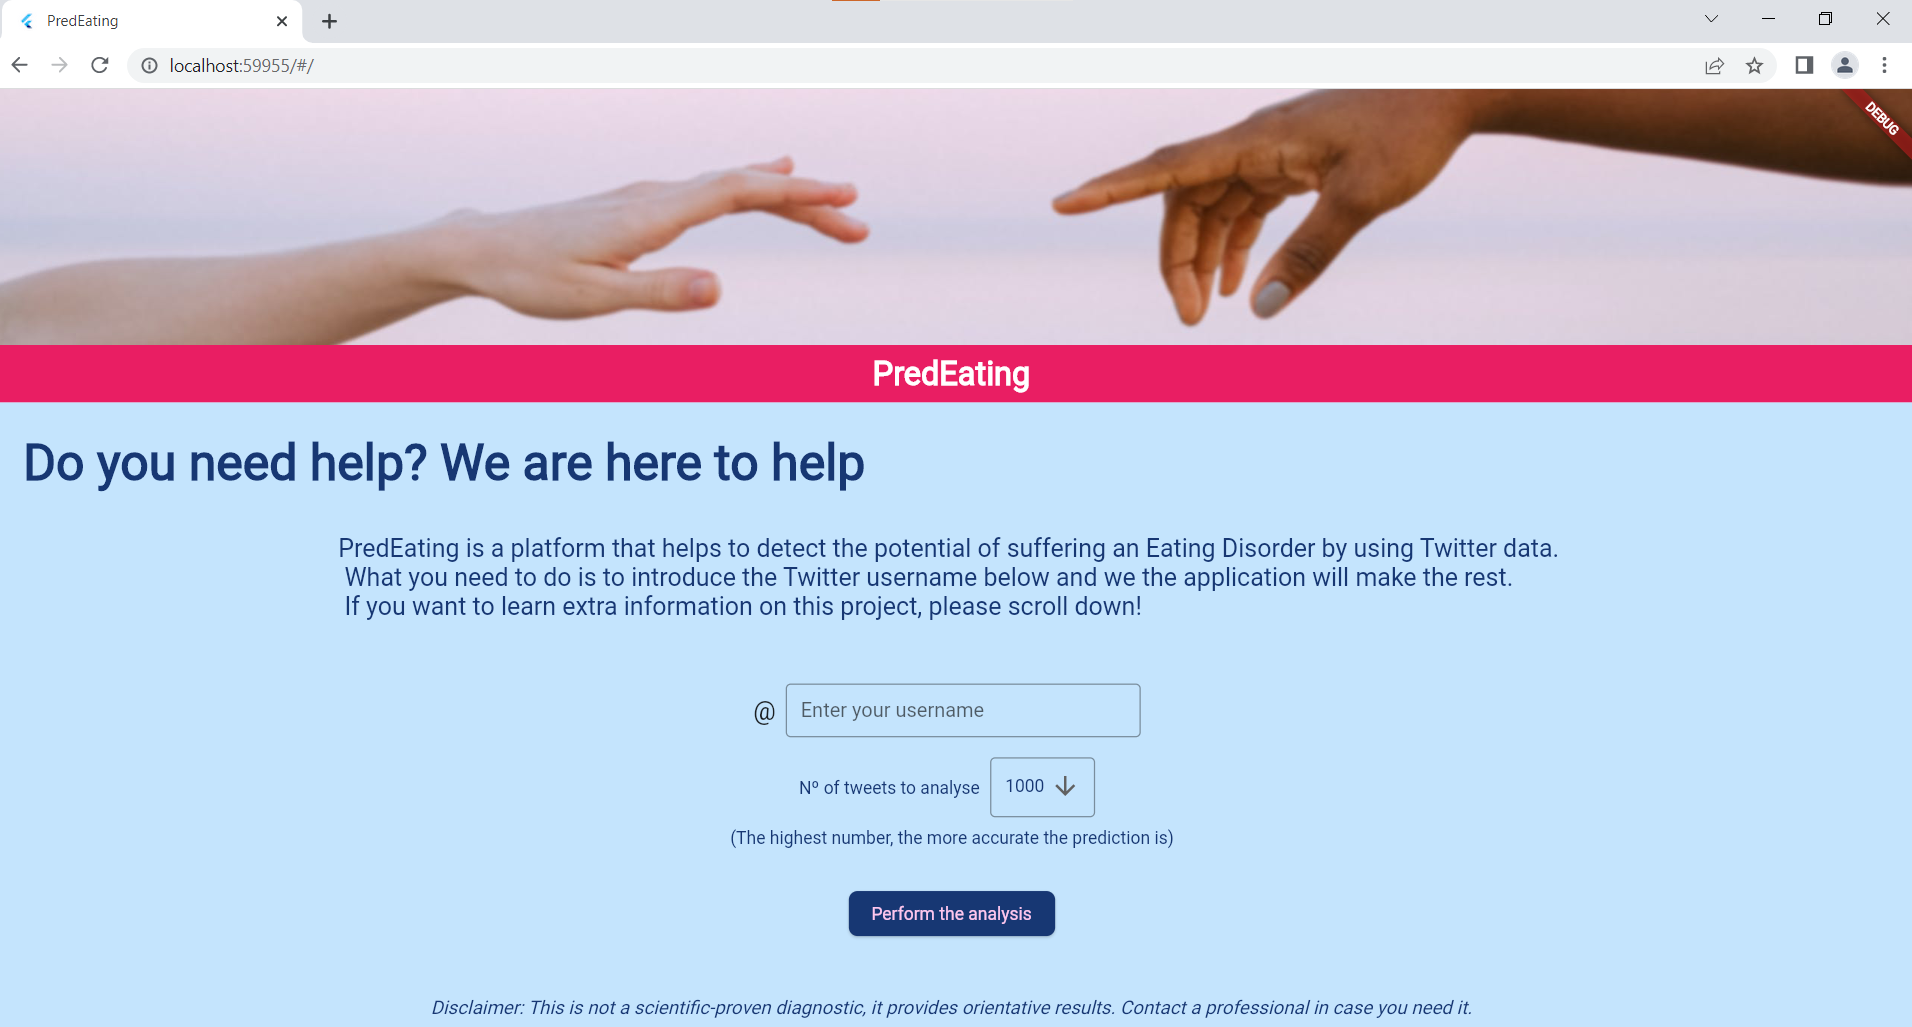
\includegraphics[scale=0.5]{img/case/landing.png}
    \caption{Landing page of PredEating}
    \label{fig:landing}
\end{figure}

As it can be seen, there is a form in the middle of the page, where the user can enter the Twitter profile to analyse. There is also another parameter which serve for modifying the number of tweets that are scrapped. If there are more, the prediction will be more accurate but on the contrary, it will take more time to process the request to the server.

There is a disclaimer since it is not a scientific-proven algorithm since it has some percentage of error. We decided to include that since the information and the prediction are sensitive information that must be treated with a lot of responsability.

The page is public and open because there is no need to log in for using the platform. We designed it this way because we wanted it to be a social contribution without the need of having to authenticate to get access to the prediction.

\myparagraph{Prediction Screen}
This screen is the one which shows the results of the prediction. While the request is being processed, the page shows a loading icon and when the response from the server is received the page from the Figure~\ref{fig:predictionscreen} is shown.

\begin{figure}[!htp]
    \centering
    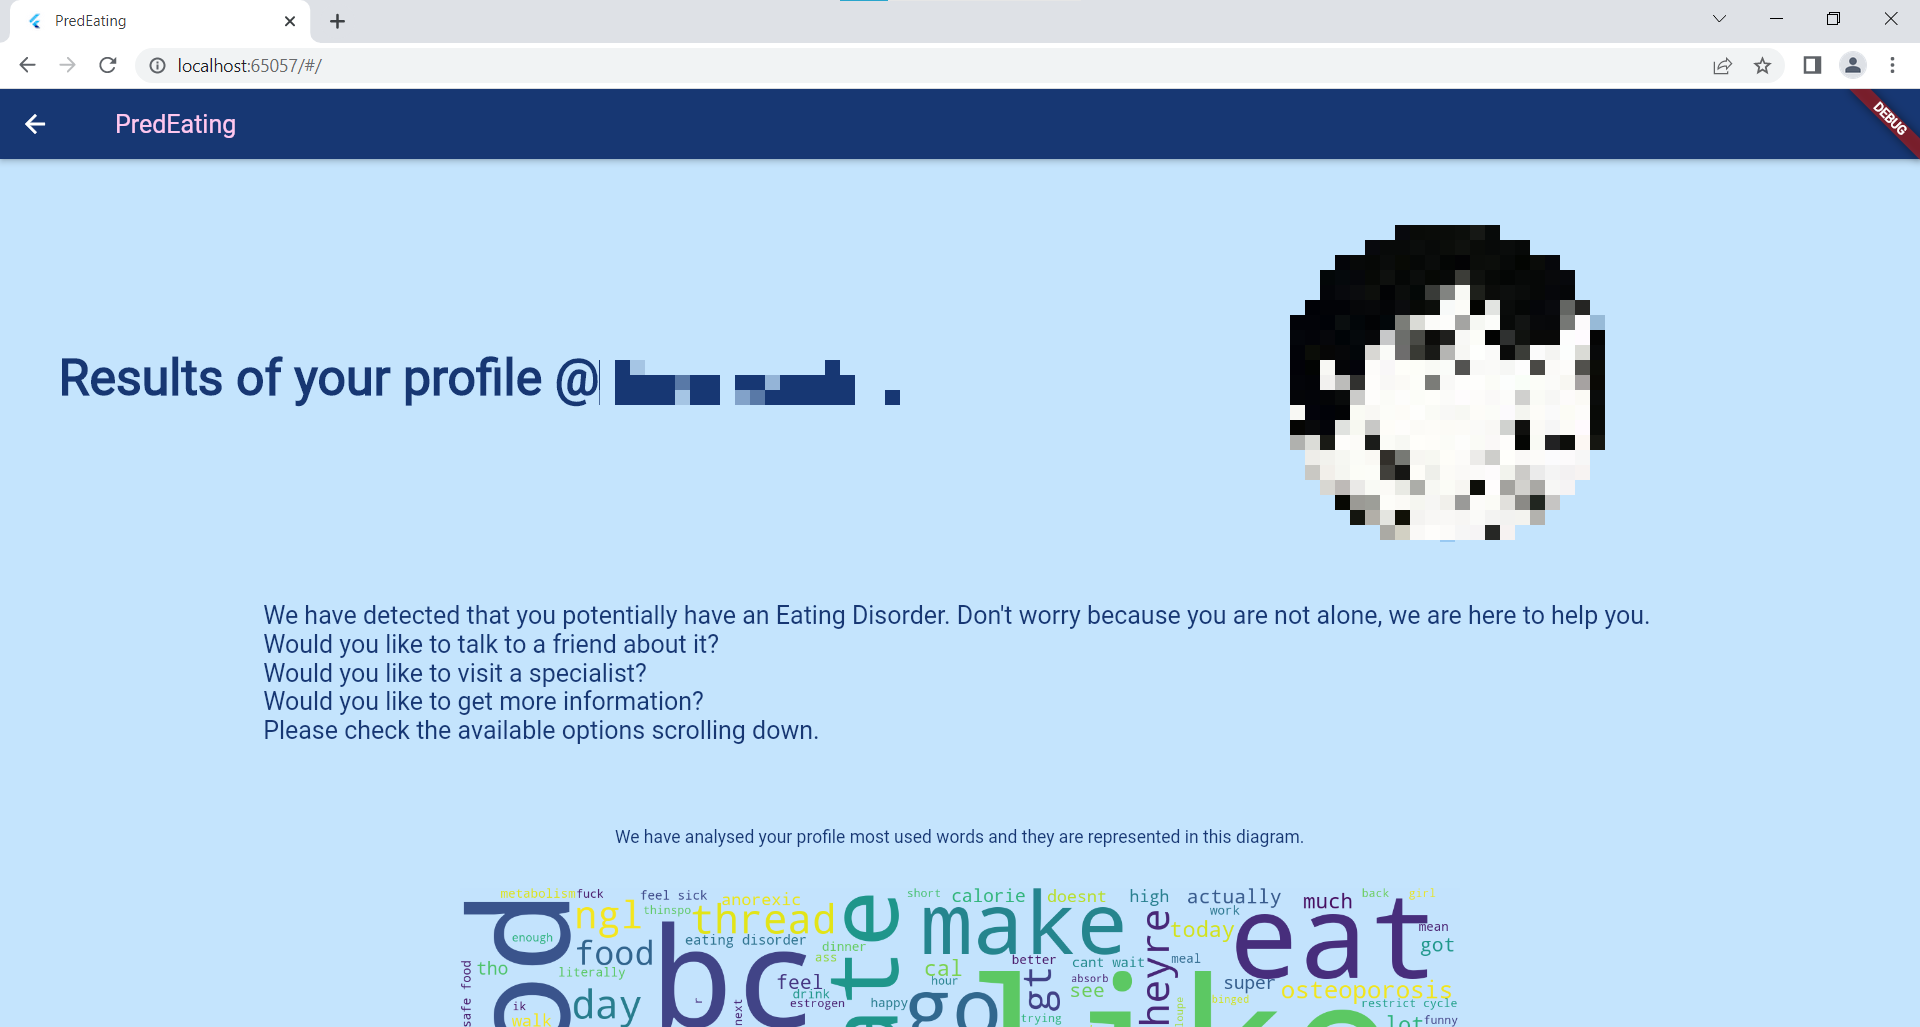
\includegraphics[scale=0.5]{img/case/predictionscreen.png}
    \caption{Prediction screen}
    \label{fig:predictionscreen}
\end{figure}

On it we can see the identifier and profile picture of the person which has been analysed. Afterwards, the prediction is shown, which can prompt either a positive prediction result or a negative one. In case of the negative, nothing else is performed on the screen.

In case the prediction is positive, we have implemented the Task Automation Service which triggers an event against it. The actions that the user can take have been defined thinking on what could be useful in this situation. The possible choices the user could have are:
\begin{itemize}
    \item Contacting one of the closest friends from Twitter that this user has.
    \item Contacting an organization that is focused on treating Eating Disorders.
    \item Contacting a professional for having a medical appointment.
\end{itemize}

There is also one button that can be clicked by all the users independently of the result of the prediction which serve for going to the third screen.

\myparagraph{Comparation Screen}
Here all the users could select another user profile from Twitter that can analyse and compare the most relevant information. The purpose of it is to give the user the possibility of having additional information and comparison with other users.




